% !TEX encoding = UTF-8 Unicode
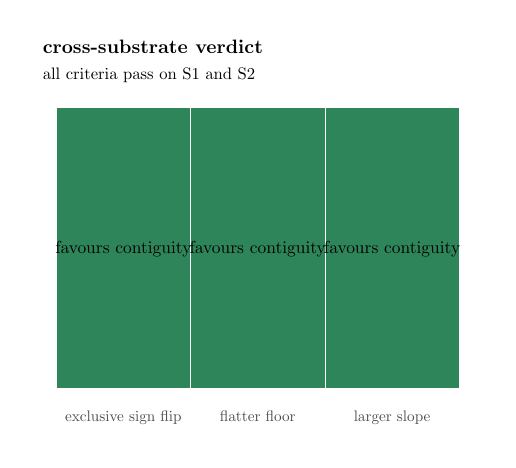
\begin{tikzpicture}[x=1pt,y=1pt]
\definecolor{fillColor}{RGB}{255,255,255}
\path[use as bounding box,fill=fillColor,fill opacity=0.00] (0,0) rectangle (166.27,148.95);
\begin{scope}
\path[clip] (  1.45,  1.65) rectangle (164.83,147.30);
\definecolor{fillColor}{RGB}{255,255,255}

\path[fill=fillColor] (  1.45,  1.65) rectangle (164.83,147.30);
\end{scope}
\begin{scope}
\path[clip] (  5.45, 13.45) rectangle (160.83,125.47);
\definecolor{drawColor}{RGB}{255,255,255}
\definecolor{fillColor}{RGB}{47,133,90}

\path[draw=drawColor,line width= 0.1pt,fill=fillColor] (107.41, 18.54) rectangle (155.97,120.37);

\path[draw=drawColor,line width= 0.1pt,fill=fillColor] ( 10.30, 18.54) rectangle ( 58.86,120.37);

\path[draw=drawColor,line width= 0.1pt,fill=fillColor] ( 58.86, 18.54) rectangle (107.41,120.37);
\definecolor{drawColor}{RGB}{0,0,0}

\node[text=drawColor,anchor=base,inner sep=0pt, outer sep=0pt, scale=  0.63] at (131.69, 67.30) {favours contiguity};

\node[text=drawColor,anchor=base,inner sep=0pt, outer sep=0pt, scale=  0.63] at ( 34.58, 67.30) {favours contiguity};

\node[text=drawColor,anchor=base,inner sep=0pt, outer sep=0pt, scale=  0.63] at ( 83.14, 67.30) {favours contiguity};
\end{scope}
\begin{scope}
\path[clip] (  0.00,  0.00) rectangle (166.27,148.95);
\definecolor{drawColor}{gray}{0.30}

\node[text=drawColor,anchor=base,inner sep=0pt, outer sep=0pt, scale=  0.55] at ( 34.58,  6.51) {exclusive sign flip};

\node[text=drawColor,anchor=base,inner sep=0pt, outer sep=0pt, scale=  0.55] at ( 83.14,  6.51) {flatter floor};

\node[text=drawColor,anchor=base,inner sep=0pt, outer sep=0pt, scale=  0.55] at (131.69,  6.51) {larger slope};
\end{scope}
\begin{scope}
\path[clip] (  0.00,  0.00) rectangle (166.27,148.95);
\definecolor{drawColor}{RGB}{0,0,0}

\node[text=drawColor,anchor=base west,inner sep=0pt, outer sep=0pt, scale=  0.60] at (  5.45,130.29) {all criteria pass on S1 and S2};
\end{scope}
\begin{scope}
\path[clip] (  0.00,  0.00) rectangle (166.27,148.95);
\definecolor{drawColor}{RGB}{0,0,0}

\node[text=drawColor,anchor=base west,inner sep=0pt, outer sep=0pt, scale=  0.70] at (  5.45,139.47) {\bfseries cross-substrate verdict};
\end{scope}
\end{tikzpicture}
